\documentclass[man]{apa6}
\usepackage{lmodern}
\usepackage{amssymb,amsmath}
\usepackage{ifxetex,ifluatex}
\usepackage{fixltx2e} % provides \textsubscript
\ifnum 0\ifxetex 1\fi\ifluatex 1\fi=0 % if pdftex
  \usepackage[T1]{fontenc}
  \usepackage[utf8]{inputenc}
\else % if luatex or xelatex
  \ifxetex
    \usepackage{mathspec}
  \else
    \usepackage{fontspec}
  \fi
  \defaultfontfeatures{Ligatures=TeX,Scale=MatchLowercase}
\fi
% use upquote if available, for straight quotes in verbatim environments
\IfFileExists{upquote.sty}{\usepackage{upquote}}{}
% use microtype if available
\IfFileExists{microtype.sty}{%
\usepackage{microtype}
\UseMicrotypeSet[protrusion]{basicmath} % disable protrusion for tt fonts
}{}
\usepackage{hyperref}
\hypersetup{unicode=true,
            pdftitle={Maternal Emotion Dysregulation and its Association with Child Internalizing and Externalizing Behaviors and Heart Rate Variability},
            pdfauthor={Jackie O'Brien, Jenn Lewis, \& Yoel Everett},
            pdfkeywords={emotion regulation, parenting, child outcomes},
            pdfborder={0 0 0},
            breaklinks=true}
\urlstyle{same}  % don't use monospace font for urls
\usepackage{graphicx,grffile}
\makeatletter
\def\maxwidth{\ifdim\Gin@nat@width>\linewidth\linewidth\else\Gin@nat@width\fi}
\def\maxheight{\ifdim\Gin@nat@height>\textheight\textheight\else\Gin@nat@height\fi}
\makeatother
% Scale images if necessary, so that they will not overflow the page
% margins by default, and it is still possible to overwrite the defaults
% using explicit options in \includegraphics[width, height, ...]{}
\setkeys{Gin}{width=\maxwidth,height=\maxheight,keepaspectratio}
\IfFileExists{parskip.sty}{%
\usepackage{parskip}
}{% else
\setlength{\parindent}{0pt}
\setlength{\parskip}{6pt plus 2pt minus 1pt}
}
\setlength{\emergencystretch}{3em}  % prevent overfull lines
\providecommand{\tightlist}{%
  \setlength{\itemsep}{0pt}\setlength{\parskip}{0pt}}
\setcounter{secnumdepth}{0}
% Redefines (sub)paragraphs to behave more like sections
\ifx\paragraph\undefined\else
\let\oldparagraph\paragraph
\renewcommand{\paragraph}[1]{\oldparagraph{#1}\mbox{}}
\fi
\ifx\subparagraph\undefined\else
\let\oldsubparagraph\subparagraph
\renewcommand{\subparagraph}[1]{\oldsubparagraph{#1}\mbox{}}
\fi

%%% Use protect on footnotes to avoid problems with footnotes in titles
\let\rmarkdownfootnote\footnote%
\def\footnote{\protect\rmarkdownfootnote}


  \title{Maternal Emotion Dysregulation and its Association with Child
Internalizing and Externalizing Behaviors and Heart Rate Variability}
    \author{Jackie O'Brien\textsuperscript{1}, Jenn Lewis\textsuperscript{1}, \&
Yoel Everett\textsuperscript{1}}
    \date{}
  
\shorttitle{Maternal Emotion Dysregulation and Child Outcomes}
\affiliation{
\vspace{0.5cm}
\textsuperscript{1} University of Oregon}
\keywords{emotion regulation, parenting, child outcomes\newline\indent Word count: X}
\usepackage{csquotes}
\usepackage{upgreek}
\captionsetup{font=singlespacing,justification=justified}

\usepackage{longtable}
\usepackage{lscape}
\usepackage{multirow}
\usepackage{tabularx}
\usepackage[flushleft]{threeparttable}
\usepackage{threeparttablex}

\newenvironment{lltable}{\begin{landscape}\begin{center}\begin{ThreePartTable}}{\end{ThreePartTable}\end{center}\end{landscape}}

\makeatletter
\newcommand\LastLTentrywidth{1em}
\newlength\longtablewidth
\setlength{\longtablewidth}{1in}
\newcommand{\getlongtablewidth}{\begingroup \ifcsname LT@\roman{LT@tables}\endcsname \global\longtablewidth=0pt \renewcommand{\LT@entry}[2]{\global\advance\longtablewidth by ##2\relax\gdef\LastLTentrywidth{##2}}\@nameuse{LT@\roman{LT@tables}} \fi \endgroup}


\DeclareDelayedFloatFlavor{ThreePartTable}{table}
\DeclareDelayedFloatFlavor{lltable}{table}
\DeclareDelayedFloatFlavor*{longtable}{table}
\makeatletter
\renewcommand{\efloat@iwrite}[1]{\immediate\expandafter\protected@write\csname efloat@post#1\endcsname{}}
\makeatother
\usepackage{lineno}

\linenumbers

\authornote{

Correspondence concerning this article should be addressed to Jackie
O'Brien, Postal address. E-mail:
\href{mailto:my@email.com}{\nolinkurl{my@email.com}}}

\abstract{
One or two sentences providing a \textbf{basic introduction} to the
field, comprehensible to a scientist in any discipline.

Two to three sentences of \textbf{more detailed background},
comprehensible to scientists in related disciplines.

One sentence clearly stating the \textbf{general problem} being
addressed by this particular study.

One sentence summarizing the main result (with the words ``\textbf{here
we show}'' or their equivalent).

Two or three sentences explaining what the \textbf{main result} reveals
in direct comparison to what was thought to be the case previously, or
how the main result adds to previous knowledge.

One or two sentences to put the results into a more \textbf{general
context}.

Two or three sentences to provide a \textbf{broader perspective},
readily comprehensible to a scientist in any discipline.


}

\begin{document}
\maketitle

\begin{verbatim}
## Observations: 97
## Variables: 6
## $ family_id      <dbl> 1001, 1002, 1003, 1004, 1005, 1006, 1007, 1008,...
## $ cbcl_int       <dbl> 10, 4, 15, 9, 10, 10, 5, 4, 3, 6, 3, 10, 13, 5,...
## $ cbcl_ext       <dbl> 13, 12, 20, 14, 18, 16, 7, 12, 3, 6, 0, 7, 17, ...
## $ ders           <dbl> 54, 59, 87, 75, 48, 65, 55, 53, 54, 48, 40, 68,...
## $ child_baseline <dbl> 7.038787, 5.819146, NA, 5.684124, NA, NA, 6.111...
## $ child_lego     <dbl> 5.952458, 5.132448, 6.669899, 4.372479, 5.04177...
\end{verbatim}

\begin{verbatim}
## Observations: 136
## Variables: 6
## $ family_id      <dbl> 1001, 1002, 1003, 1004, 1005, 1006, 1007, 1008,...
## $ ders           <dbl> 54, 59, 87, 75, 48, 65, 55, 53, 54, 48, 40, 68,...
## $ child_baseline <dbl> 7.038787, 5.819146, NA, 5.684124, NA, NA, 6.111...
## $ child_lego     <dbl> 5.952458, 5.132448, 6.669899, 4.372479, 5.04177...
## $ cbcl_subtype   <chr> "int", "int", "int", "int", "int", "int", "int"...
## $ cbcl_score     <dbl> 10, 4, 15, 9, 10, 10, 5, 4, 3, 6, 3, 10, 13, 5,...
\end{verbatim}

\begin{verbatim}
## Observations: 136
## Variables: 9
## $ family_id      <dbl> 1001, 1002, 1003, 1004, 1005, 1006, 1007, 1008,...
## $ ders           <dbl> 54, 59, 87, 75, 48, 65, 55, 53, 54, 48, 40, 68,...
## $ child_baseline <dbl> 7.038787, 5.819146, NA, 5.684124, NA, NA, 6.111...
## $ child_lego     <dbl> 5.952458, 5.132448, 6.669899, 4.372479, 5.04177...
## $ cbcl_subtype   <chr> "int", "int", "int", "int", "int", "int", "int"...
## $ cbcl_score     <dbl> 10, 4, 15, 9, 10, 10, 5, 4, 3, 6, 3, 10, 13, 5,...
## $ reactivity     <dbl> -1.086328857, -0.686697786, NA, -1.311645429, N...
## $ ders_c         <dbl> -16.102941, -11.102941, 16.897059, 4.897059, -2...
## $ reactivity_c   <dbl> 0.014032141, 0.413663212, NA, -0.211284431, NA,...
\end{verbatim}

\section{Introduction}\label{introduction}

\section{Methods}\label{methods}

We report how we determined our sample size, all data exclusions (if
any), all manipulations, and all measures in the study.

\subsection{Participants}\label{participants}

\subsection{Material}\label{material}

\subsection{Procedure}\label{procedure}

\subsection{Data analysis}\label{data-analysis}

We used R (Version 3.5.1; R Core Team, 2018) and the R-packages
\emph{bindrcpp} (Version 0.2.2; Müller, 2018), \emph{dplyr} (Version
0.7.7; Wickham, François, Henry, \& Müller, 2018), \emph{forcats}
(Version 0.3.0; Wickham, 2018a), \emph{ggplot2} (Version 3.0.0; Wickham,
2016), \emph{here} (Version 0.1; Müller, 2017), \emph{kableExtra}
(Version 0.9.0; Zhu, 2018), \emph{papaja} (Version 0.1.0.9842; Aust \&
Barth, 2018), \emph{purrr} (Version 0.2.5; Henry \& Wickham, 2018),
\emph{readr} (Version 1.1.1; Wickham, Hester, \& Francois, 2017),
\emph{rio} (Version 0.5.10; C.-h. Chan, Chan, Leeper, \& Becker, 2018),
\emph{stringr} (Version 1.3.1; Wickham, 2018b), \emph{tibble} (Version
1.4.2; Müller \& Wickham, 2018), \emph{tidyr} (Version 0.8.1; Wickham \&
Henry, 2018), and \emph{tidyverse} (Version 1.2.1; Wickham, 2017) for
all our analyses.

\section{Results}\label{results}

\begin{verbatim}
## 'data.frame':    136 obs. of  9 variables:
##  $ family_id     : num  1001 1002 1003 1004 1005 ...
##  $ ders          : num  54 59 87 75 48 65 55 53 54 48 ...
##  $ child_baseline: num  7.04 5.82 NA 5.68 NA ...
##  $ child_lego    : num  5.95 5.13 6.67 4.37 5.04 ...
##  $ cbcl_subtype  : chr  "int" "int" "int" "int" ...
##  $ cbcl_score    : num  10 4 15 9 10 10 5 4 3 6 ...
##  $ reactivity    : num  -1.086 -0.687 NA -1.312 NA ...
##  $ ders_c        : num  -16.1 -11.1 16.9 4.9 -22.1 ...
##  $ reactivity_c  : num  0.014 0.414 NA -0.211 NA ...
\end{verbatim}

\begin{tabular}{rrrr}
\toprule
DERS\_mean & DERS\_SD & Reactivity\_mean & Reactivity\_SD\\
\midrule
70.10294 & 22.33027 & -1.100361 & 0.6520285\\
\bottomrule
\end{tabular}

\begin{tabular}{lrr}
\toprule
cbcl\_subtype & cbcl\_mean & cbcl\_SD\\
\midrule
ext & 16.28333 & 9.492662\\
int & 11.17318 & 7.539277\\
\bottomrule
\end{tabular}

\begin{verbatim}
## 
## Call:
## lm(formula = cbcl_score ~ ders_c * reactivity_c, data = subset(tidy_data, 
##     cbcl_subtype == "int"))
## 
## Residuals:
##    Min     1Q Median     3Q    Max 
## -9.871 -4.287 -1.288  2.292 17.350 
## 
## Coefficients:
##                     Estimate Std. Error t value Pr(>|t|)    
## (Intercept)         11.00475    0.97629  11.272 1.07e-14 ***
## ders_c               0.16504    0.04142   3.985 0.000245 ***
## reactivity_c        -1.19234    1.54053  -0.774 0.442990    
## ders_c:reactivity_c -0.18142    0.07985  -2.272 0.027927 *  
## ---
## Signif. codes:  0 '***' 0.001 '**' 0.01 '*' 0.05 '.' 0.1 ' ' 1
## 
## Residual standard error: 6.814 on 45 degrees of freedom
##   (19 observations deleted due to missingness)
## Multiple R-squared:  0.3413, Adjusted R-squared:  0.2974 
## F-statistic: 7.772 on 3 and 45 DF,  p-value: 0.0002752
\end{verbatim}

\begin{verbatim}
## 
## Call:
## lm(formula = cbcl_score ~ ders_c * reactivity_c, data = subset(tidy_data, 
##     cbcl_subtype == "ext"))
## 
## Residuals:
##     Min      1Q  Median      3Q     Max 
## -11.938  -6.341  -2.041   3.818  27.750 
## 
## Coefficients:
##                     Estimate Std. Error t value Pr(>|t|)    
## (Intercept)         16.01973    1.32811  12.062 1.07e-15 ***
## ders_c               0.16025    0.05634   2.844  0.00668 ** 
## reactivity_c         1.72370    2.09567   0.823  0.41513    
## ders_c:reactivity_c -0.03287    0.10863  -0.303  0.76360    
## ---
## Signif. codes:  0 '***' 0.001 '**' 0.01 '*' 0.05 '.' 0.1 ' ' 1
## 
## Residual standard error: 9.27 on 45 degrees of freedom
##   (19 observations deleted due to missingness)
## Multiple R-squared:  0.1698, Adjusted R-squared:  0.1144 
## F-statistic: 3.068 on 3 and 45 DF,  p-value: 0.03733
\end{verbatim}

\begin{verbatim}
## Warning: Removed 4 rows containing non-finite values (stat_smooth).
\end{verbatim}

\begin{verbatim}
## Warning: Removed 4 rows containing missing values (geom_point).
\end{verbatim}

\begin{figure}
\centering
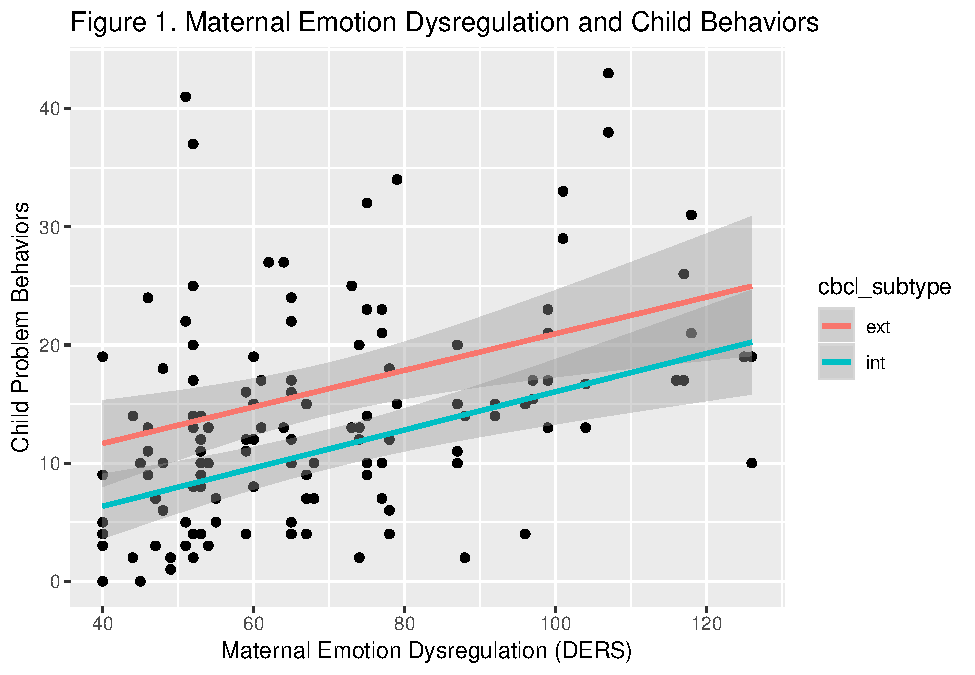
\includegraphics{DataPrepScript_apa_style_files/figure-latex/plots-1.pdf}
\caption{}
\end{figure}

\begin{verbatim}
## Warning: Removed 36 rows containing non-finite values (stat_smooth).
\end{verbatim}

\begin{verbatim}
## Warning: Removed 36 rows containing missing values (geom_point).
\end{verbatim}

\begin{figure}
\centering
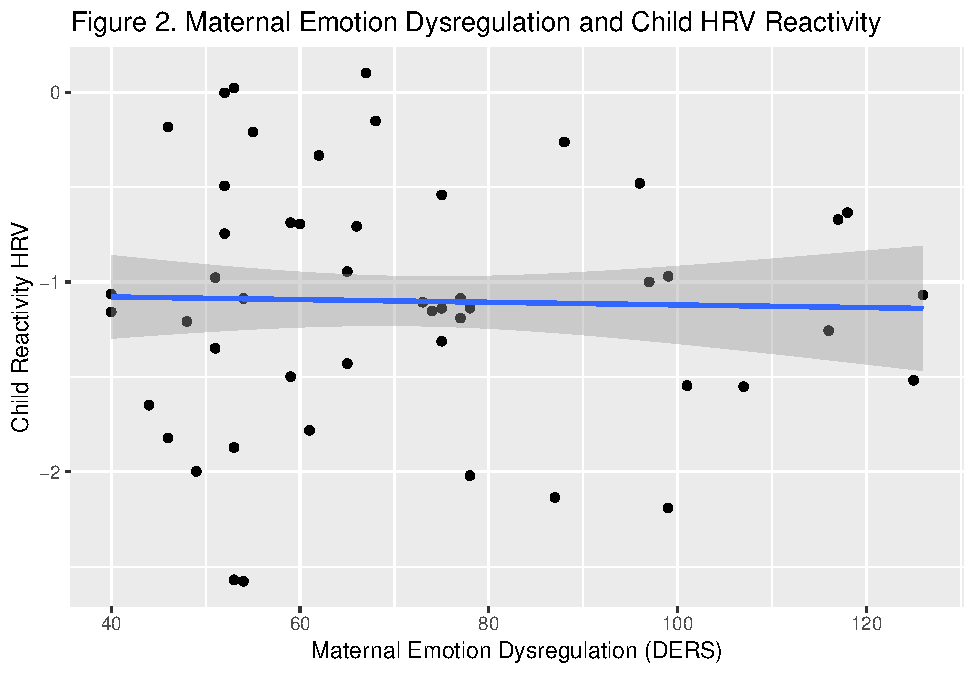
\includegraphics{DataPrepScript_apa_style_files/figure-latex/plots-2.pdf}
\caption{}
\end{figure}

\section{Discussion}\label{discussion}

\newpage

\section{References}\label{references}

\begingroup
\setlength{\parindent}{-0.5in} \setlength{\leftskip}{0.5in}

\hypertarget{refs}{}
\hypertarget{ref-R-papaja}{}
Aust, F., \& Barth, M. (2018). \emph{papaja: Create APA manuscripts with
R Markdown}. Retrieved from \url{https://github.com/crsh/papaja}

\hypertarget{ref-R-rio}{}
Chan, C.-h., Chan, G. C., Leeper, T. J., \& Becker, J. (2018).
\emph{Rio: A swiss-army knife for data file i/o}.

\hypertarget{ref-R-purrr}{}
Henry, L., \& Wickham, H. (2018). \emph{Purrr: Functional programming
tools}. Retrieved from \url{https://CRAN.R-project.org/package=purrr}

\hypertarget{ref-R-here}{}
Müller, K. (2017). \emph{Here: A simpler way to find your files}.
Retrieved from \url{https://CRAN.R-project.org/package=here}

\hypertarget{ref-R-bindrcpp}{}
Müller, K. (2018). \emph{Bindrcpp: An 'rcpp' interface to active
bindings}. Retrieved from
\url{https://CRAN.R-project.org/package=bindrcpp}

\hypertarget{ref-R-tibble}{}
Müller, K., \& Wickham, H. (2018). \emph{Tibble: Simple data frames}.
Retrieved from \url{https://CRAN.R-project.org/package=tibble}

\hypertarget{ref-R-base}{}
R Core Team. (2018). \emph{R: A language and environment for statistical
computing}. Vienna, Austria: R Foundation for Statistical Computing.
Retrieved from \url{https://www.R-project.org/}

\hypertarget{ref-R-ggplot2}{}
Wickham, H. (2016). \emph{Ggplot2: Elegant graphics for data analysis}.
Springer-Verlag New York. Retrieved from \url{http://ggplot2.org}

\hypertarget{ref-R-tidyverse}{}
Wickham, H. (2017). \emph{Tidyverse: Easily install and load the
'tidyverse'}. Retrieved from
\url{https://CRAN.R-project.org/package=tidyverse}

\hypertarget{ref-R-forcats}{}
Wickham, H. (2018a). \emph{Forcats: Tools for working with categorical
variables (factors)}. Retrieved from
\url{https://CRAN.R-project.org/package=forcats}

\hypertarget{ref-R-stringr}{}
Wickham, H. (2018b). \emph{Stringr: Simple, consistent wrappers for
common string operations}. Retrieved from
\url{https://CRAN.R-project.org/package=stringr}

\hypertarget{ref-R-tidyr}{}
Wickham, H., \& Henry, L. (2018). \emph{Tidyr: Easily tidy data with
'spread()' and 'gather()' functions}. Retrieved from
\url{https://CRAN.R-project.org/package=tidyr}

\hypertarget{ref-R-dplyr}{}
Wickham, H., François, R., Henry, L., \& Müller, K. (2018). \emph{Dplyr:
A grammar of data manipulation}. Retrieved from
\url{https://CRAN.R-project.org/package=dplyr}

\hypertarget{ref-R-readr}{}
Wickham, H., Hester, J., \& Francois, R. (2017). \emph{Readr: Read
rectangular text data}. Retrieved from
\url{https://CRAN.R-project.org/package=readr}

\hypertarget{ref-R-kableExtra}{}
Zhu, H. (2018). \emph{KableExtra: Construct complex table with 'kable'
and pipe syntax}. Retrieved from
\url{https://CRAN.R-project.org/package=kableExtra}

\endgroup


\end{document}
